\documentclass[paper=a4, fontsize=11pt]{article}

%----------------------------------------------------------------------------------------
%	PACKAGES AND OTHER DOCUMENT CONFIGURATIONS
%----------------------------------------------------------------------------------------

\usepackage{amsmath,amsfonts,amsthm} % Math packages
\usepackage{sectsty} % Allows customizing section commands
\allsectionsfont{\centering \normalfont\scshape} % Make all sections centered, the default font and small caps

\usepackage{fancyhdr} % Custom headers and footers
\pagestyle{fancyplain} % Makes all pages in the document conform to the custom headers and footers
\fancyhead{} % No page header - if you want one, create it in the same way as the footers below
\fancyfoot[L]{} % Empty left footer
\fancyfoot[C]{} % Empty center footer
\fancyfoot[R]{\thepage} % Page numbering for right footer
\renewcommand{\headrulewidth}{0pt} % Remove header underlines
\renewcommand{\footrulewidth}{0pt} % Remove footer underlines
\setlength{\headheight}{13.6pt} % Customize the height of the header

\numberwithin{equation}{section} % Number equations within sections (i.e. 1.1, 1.2, 2.1, 2.2 instead of 1, 2, 3, 4)
\numberwithin{figure}{section} % Number figures within sections (i.e. 1.1, 1.2, 2.1, 2.2 instead of 1, 2, 3, 4)
\numberwithin{table}{section} % Number tables within sections (i.e. 1.1, 1.2, 2.1, 2.2 instead of 1, 2, 3, 4)

\setlength\parindent{0pt} % Removes all indentation from paragraphs - comment this line for an assignment with lots of text

\usepackage{tikz-qtree}
\usepackage{lscape}

\usepackage{graphicx}
\graphicspath{ {images/} }

\usepackage{xepersian}
\settextfont[Path=fonts/]{Vazir.ttf}
%\setlatintextfont{Times New Roman}

%----------------------------------------------------------------------------------------
%	TITLE SECTION
%----------------------------------------------------------------------------------------

\newcommand{\horrule}[1]{\rule{\linewidth}{#1}} % Create horizontal rule command with 1 argument of height

\title{
\normalfont\normalsize

\includegraphics[scale=0.1]{aut}
\hspace{5cm}

\includegraphics[scale=0.1]{ceit} \\
\textsc دانشگاه صنعتی امیرکبیر \\
\textsc دانشکده مهندسی کامپیوتر و فناوری اطلاعات
\horrule{0.5pt} \\ [0.4cm] % Thin top horizontal rule
\huge معماری سوئیچ و روترهای با کارآیی بالا \\ % The assignment title
\huge تمرین اول \\ % The assignment title
\horrule{2pt} \\ [0.5cm] % Thick bottom horizontal rule
}

\author{پرهام الوانی}

\date{\normalsize\today} % Today's date or a custom date

\begin{document}

\maketitle % Print the title

\section{سوال اول}
\par
هر عنصر می‌تواند در هر یک از ۱۰۰۰۰ بلوک موجود قرار بگیرد.
فرض می‌کنیم یکی از ۱۰۰۰۰ بلوک خالی باشد، به این ترتیب هر عنصر ۹۹۹۹ انتخاب خواهد داشت.
بنابراین احتمال خالی بودن یکی از بلوک‌ها به شرح زیر است:


\begin{align}
\begin{split}
    \frac{\binom{10^4}{1} * (10^4-1)^{5000}}{10^{4^{5000}}}
\end{split}
\end{align}

\par
اگر فرض کنیم متغیر تصادفی x نشان‌دهنده‌ی تعداد بلوک‌های خالی باشد،
امید ریاضی x متوسط تعداد بلوک‌های خالی خواهد بود
به این ترتیب داریم:

\begin{align}
\begin{split}
    E[x] = \sum_{n = 0}^{10^4}n\frac{\binom{10^4}{n} * (10^4-1)^{5000}}{10^{4^{5000}}}
\end{split}
\end{align}

\section{سوال دوم}
\par
برای جستجو در اولین گام بلوک مورد نظر مشخص می‌شود و سپس جستجو در همان بلوک صورت می‌پذیرد.
از آنجایی که جستجو در بلوک صورت می‌پذیرد پس زمان آن به اندازه‌ی بلوک وابسته است،
اندازه‌ی هر بلوک در صورتی که تعداد عناصر آن‌ها با یکدیگر برابر باشد
$n/m$
می‌باشد.

$$
search = O(n/m)
$$

\par
حافظه‌ی مصرفی این روش اگر تعداد عناصر همه‌ی بلوک‌ها با یکدیگر برابر باشد
به اندازه‌ی عناصر موجود خواهد بود ولی
در صورتی که این امر اتفاق نیافتد
حافظه‌ی مصرفی این روش از تعداد عناصر موجود بیشتر خواهد بود.

$$
memroy = \Omega(n/m)
$$

\section{سوال سوم}

\begin{landscape}
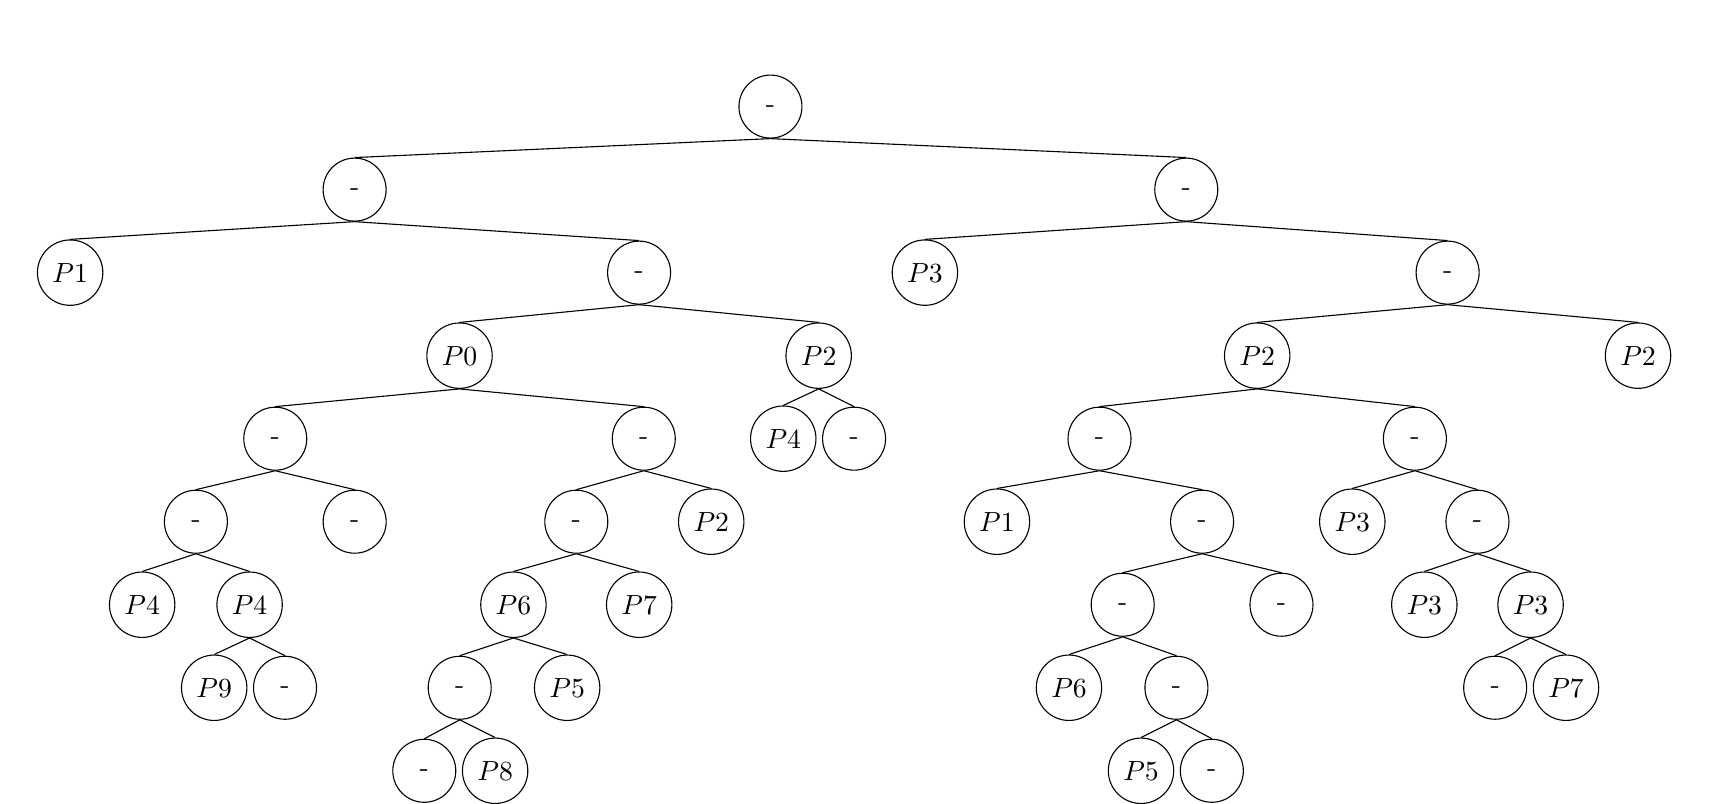
\begin{tikzpicture}[every tree node/.style={draw, circle, minimum width=0.8cm}]
    \matrix{
        \Tree
        [.-
            % 0
            [.- 
                % 00
                [.$P1$ ]
                % 01
                [.- 
                    % 010
                    [.$P0$
                        % 010 0
                        [.-
                            % 010 00
                            [.- $P4$
                                [.$P4$ $P9$ - ]
                            ]
                            % 010 01
                            [.- ]
                        ]
                        % 010 1
                        [.-
                            % 010 10
                            [.- 
                                [.$P6$
                                    [.- - $P8$ ]
                                    [.$P5$ ]
                                ]
                                [.$P7$ ]
                            ]
                            % 010 11
                            [.$P2$ ]
                        ]
                    ]
                    % 011
                    [.$P2$ $P4$ - ]
                ]
            ]
            % 1
            [.-
                % 10
                [.$P3$ ]
                % 11
                [.-
                    % 110
                    [.$P2$
                        % 110 0
                        [.-
                            % 110 00
                            [.$P1$ ]
                            % 110 01
                            [.-
                                % 110 010
                                [.-
                                    [.$P6$ ]
                                    [.- $P5$ - ]
                                ]
                                % 110 011
                                [.- ]
                            ]
                        ]
                        % 110 1
                        [.-
                            % 110 10
                            [.$P3$ ]
                            % 110 11
                            [.-
                                [.$P3$ ]
                                [.$P3$ - $P7$ ]
                            ]
                        ]
                    ]
                    [.$P2$ ]
                ]
            ]
        ]
        &
    \\};
\end{tikzpicture}
\end{landscape}

\section{سوال چهارم}

\end{document}
